% Options for packages loaded elsewhere
\PassOptionsToPackage{unicode}{hyperref}
\PassOptionsToPackage{hyphens}{url}
%
\documentclass[
]{article}
\usepackage{amsmath,amssymb}
\usepackage{lmodern}
\usepackage{ifxetex,ifluatex}
\ifnum 0\ifxetex 1\fi\ifluatex 1\fi=0 % if pdftex
  \usepackage[T1]{fontenc}
  \usepackage[utf8]{inputenc}
  \usepackage{textcomp} % provide euro and other symbols
\else % if luatex or xetex
  \usepackage{unicode-math}
  \defaultfontfeatures{Scale=MatchLowercase}
  \defaultfontfeatures[\rmfamily]{Ligatures=TeX,Scale=1}
\fi
% Use upquote if available, for straight quotes in verbatim environments
\IfFileExists{upquote.sty}{\usepackage{upquote}}{}
\IfFileExists{microtype.sty}{% use microtype if available
  \usepackage[]{microtype}
  \UseMicrotypeSet[protrusion]{basicmath} % disable protrusion for tt fonts
}{}
\makeatletter
\@ifundefined{KOMAClassName}{% if non-KOMA class
  \IfFileExists{parskip.sty}{%
    \usepackage{parskip}
  }{% else
    \setlength{\parindent}{0pt}
    \setlength{\parskip}{6pt plus 2pt minus 1pt}}
}{% if KOMA class
  \KOMAoptions{parskip=half}}
\makeatother
\usepackage{xcolor}
\IfFileExists{xurl.sty}{\usepackage{xurl}}{} % add URL line breaks if available
\IfFileExists{bookmark.sty}{\usepackage{bookmark}}{\usepackage{hyperref}}
\hypersetup{
  pdftitle={Class 17: Vaccination Mini Project},
  pdfauthor={Claire Chapman},
  hidelinks,
  pdfcreator={LaTeX via pandoc}}
\urlstyle{same} % disable monospaced font for URLs
\usepackage[margin=1in]{geometry}
\usepackage{color}
\usepackage{fancyvrb}
\newcommand{\VerbBar}{|}
\newcommand{\VERB}{\Verb[commandchars=\\\{\}]}
\DefineVerbatimEnvironment{Highlighting}{Verbatim}{commandchars=\\\{\}}
% Add ',fontsize=\small' for more characters per line
\usepackage{framed}
\definecolor{shadecolor}{RGB}{248,248,248}
\newenvironment{Shaded}{\begin{snugshade}}{\end{snugshade}}
\newcommand{\AlertTok}[1]{\textcolor[rgb]{0.94,0.16,0.16}{#1}}
\newcommand{\AnnotationTok}[1]{\textcolor[rgb]{0.56,0.35,0.01}{\textbf{\textit{#1}}}}
\newcommand{\AttributeTok}[1]{\textcolor[rgb]{0.77,0.63,0.00}{#1}}
\newcommand{\BaseNTok}[1]{\textcolor[rgb]{0.00,0.00,0.81}{#1}}
\newcommand{\BuiltInTok}[1]{#1}
\newcommand{\CharTok}[1]{\textcolor[rgb]{0.31,0.60,0.02}{#1}}
\newcommand{\CommentTok}[1]{\textcolor[rgb]{0.56,0.35,0.01}{\textit{#1}}}
\newcommand{\CommentVarTok}[1]{\textcolor[rgb]{0.56,0.35,0.01}{\textbf{\textit{#1}}}}
\newcommand{\ConstantTok}[1]{\textcolor[rgb]{0.00,0.00,0.00}{#1}}
\newcommand{\ControlFlowTok}[1]{\textcolor[rgb]{0.13,0.29,0.53}{\textbf{#1}}}
\newcommand{\DataTypeTok}[1]{\textcolor[rgb]{0.13,0.29,0.53}{#1}}
\newcommand{\DecValTok}[1]{\textcolor[rgb]{0.00,0.00,0.81}{#1}}
\newcommand{\DocumentationTok}[1]{\textcolor[rgb]{0.56,0.35,0.01}{\textbf{\textit{#1}}}}
\newcommand{\ErrorTok}[1]{\textcolor[rgb]{0.64,0.00,0.00}{\textbf{#1}}}
\newcommand{\ExtensionTok}[1]{#1}
\newcommand{\FloatTok}[1]{\textcolor[rgb]{0.00,0.00,0.81}{#1}}
\newcommand{\FunctionTok}[1]{\textcolor[rgb]{0.00,0.00,0.00}{#1}}
\newcommand{\ImportTok}[1]{#1}
\newcommand{\InformationTok}[1]{\textcolor[rgb]{0.56,0.35,0.01}{\textbf{\textit{#1}}}}
\newcommand{\KeywordTok}[1]{\textcolor[rgb]{0.13,0.29,0.53}{\textbf{#1}}}
\newcommand{\NormalTok}[1]{#1}
\newcommand{\OperatorTok}[1]{\textcolor[rgb]{0.81,0.36,0.00}{\textbf{#1}}}
\newcommand{\OtherTok}[1]{\textcolor[rgb]{0.56,0.35,0.01}{#1}}
\newcommand{\PreprocessorTok}[1]{\textcolor[rgb]{0.56,0.35,0.01}{\textit{#1}}}
\newcommand{\RegionMarkerTok}[1]{#1}
\newcommand{\SpecialCharTok}[1]{\textcolor[rgb]{0.00,0.00,0.00}{#1}}
\newcommand{\SpecialStringTok}[1]{\textcolor[rgb]{0.31,0.60,0.02}{#1}}
\newcommand{\StringTok}[1]{\textcolor[rgb]{0.31,0.60,0.02}{#1}}
\newcommand{\VariableTok}[1]{\textcolor[rgb]{0.00,0.00,0.00}{#1}}
\newcommand{\VerbatimStringTok}[1]{\textcolor[rgb]{0.31,0.60,0.02}{#1}}
\newcommand{\WarningTok}[1]{\textcolor[rgb]{0.56,0.35,0.01}{\textbf{\textit{#1}}}}
\usepackage{longtable,booktabs,array}
\usepackage{calc} % for calculating minipage widths
% Correct order of tables after \paragraph or \subparagraph
\usepackage{etoolbox}
\makeatletter
\patchcmd\longtable{\par}{\if@noskipsec\mbox{}\fi\par}{}{}
\makeatother
% Allow footnotes in longtable head/foot
\IfFileExists{footnotehyper.sty}{\usepackage{footnotehyper}}{\usepackage{footnote}}
\makesavenoteenv{longtable}
\usepackage{graphicx}
\makeatletter
\def\maxwidth{\ifdim\Gin@nat@width>\linewidth\linewidth\else\Gin@nat@width\fi}
\def\maxheight{\ifdim\Gin@nat@height>\textheight\textheight\else\Gin@nat@height\fi}
\makeatother
% Scale images if necessary, so that they will not overflow the page
% margins by default, and it is still possible to overwrite the defaults
% using explicit options in \includegraphics[width, height, ...]{}
\setkeys{Gin}{width=\maxwidth,height=\maxheight,keepaspectratio}
% Set default figure placement to htbp
\makeatletter
\def\fps@figure{htbp}
\makeatother
\setlength{\emergencystretch}{3em} % prevent overfull lines
\providecommand{\tightlist}{%
  \setlength{\itemsep}{0pt}\setlength{\parskip}{0pt}}
\setcounter{secnumdepth}{-\maxdimen} % remove section numbering
\ifluatex
  \usepackage{selnolig}  % disable illegal ligatures
\fi

\title{Class 17: Vaccination Mini Project}
\author{Claire Chapman}
\date{11/28/2021}

\begin{document}
\maketitle

\hypertarget{getting-started}{%
\subsection{Getting Started}\label{getting-started}}

Load your data

\begin{Shaded}
\begin{Highlighting}[]
\NormalTok{vax }\OtherTok{\textless{}{-}} \FunctionTok{read.csv}\NormalTok{(}\StringTok{"covid19vaccinesbyzipcode\_test.csv"}\NormalTok{)}
\FunctionTok{head}\NormalTok{(vax)}
\end{Highlighting}
\end{Shaded}

\begin{verbatim}
##   as_of_date zip_code_tabulation_area local_health_jurisdiction         county
## 1 2021-01-05                    92395            San Bernardino San Bernardino
## 2 2021-01-05                    93206                      Kern           Kern
## 3 2021-01-05                    91006               Los Angeles    Los Angeles
## 4 2021-01-05                    91901                 San Diego      San Diego
## 5 2021-01-05                    92230                 Riverside      Riverside
## 6 2021-01-05                    92662                    Orange         Orange
##   vaccine_equity_metric_quartile                 vem_source
## 1                              1 Healthy Places Index Score
## 2                              1 Healthy Places Index Score
## 3                              3 Healthy Places Index Score
## 4                              3 Healthy Places Index Score
## 5                              1 Healthy Places Index Score
## 6                              4 Healthy Places Index Score
##   age12_plus_population age5_plus_population persons_fully_vaccinated
## 1               35915.3                40888                       NA
## 2                1237.5                 1521                       NA
## 3               28742.7                31347                       19
## 4               15549.8                16905                       12
## 5                2320.2                 2526                       NA
## 6                2349.5                 2397                       NA
##   persons_partially_vaccinated percent_of_population_fully_vaccinated
## 1                           NA                                     NA
## 2                           NA                                     NA
## 3                          873                               0.000606
## 4                          271                               0.000710
## 5                           NA                                     NA
## 6                           NA                                     NA
##   percent_of_population_partially_vaccinated
## 1                                         NA
## 2                                         NA
## 3                                   0.027850
## 4                                   0.016031
## 5                                         NA
## 6                                         NA
##   percent_of_population_with_1_plus_dose
## 1                                     NA
## 2                                     NA
## 3                               0.028456
## 4                               0.016741
## 5                                     NA
## 6                                     NA
##                                                                redacted
## 1 Information redacted in accordance with CA state privacy requirements
## 2 Information redacted in accordance with CA state privacy requirements
## 3                                                                    No
## 4                                                                    No
## 5 Information redacted in accordance with CA state privacy requirements
## 6 Information redacted in accordance with CA state privacy requirements
\end{verbatim}

\begin{quote}
Q1. What column details the total number of people fully vaccinated?
\end{quote}

8

\begin{quote}
Q2. What column details the Zip code tabulation area?
\end{quote}

2

\begin{quote}
Q3. What is the earliest date in this dataset?
\end{quote}

2021-01-05

\begin{quote}
Q4. What is the latest date in this dataset?
\end{quote}

2021-11-23

\begin{Shaded}
\begin{Highlighting}[]
\NormalTok{skimr}\SpecialCharTok{::}\FunctionTok{skim}\NormalTok{(vax)}
\end{Highlighting}
\end{Shaded}

\begin{longtable}[]{@{}ll@{}}
\caption{Data summary}\tabularnewline
\toprule
& \\
\midrule
\endfirsthead
\toprule
& \\
\midrule
\endhead
Name & vax \\
Number of rows & 82908 \\
Number of columns & 14 \\
\_\_\_\_\_\_\_\_\_\_\_\_\_\_\_\_\_\_\_\_\_\_\_ & \\
Column type frequency: & \\
character & 5 \\
numeric & 9 \\
\_\_\_\_\_\_\_\_\_\_\_\_\_\_\_\_\_\_\_\_\_\_\_\_ & \\
Group variables & None \\
\bottomrule
\end{longtable}

\textbf{Variable type: character}

\begin{longtable}[]{@{}lrrrrrrr@{}}
\toprule
skim\_variable & n\_missing & complete\_rate & min & max & empty &
n\_unique & whitespace \\
\midrule
\endhead
as\_of\_date & 0 & 1 & 10 & 10 & 0 & 47 & 0 \\
local\_health\_jurisdiction & 0 & 1 & 0 & 15 & 235 & 62 & 0 \\
county & 0 & 1 & 0 & 15 & 235 & 59 & 0 \\
vem\_source & 0 & 1 & 15 & 26 & 0 & 3 & 0 \\
redacted & 0 & 1 & 2 & 69 & 0 & 2 & 0 \\
\bottomrule
\end{longtable}

\textbf{Variable type: numeric}

\begin{longtable}[]{@{}
  >{\raggedright\arraybackslash}p{(\columnwidth - 20\tabcolsep) * \real{0.26}}
  >{\raggedleft\arraybackslash}p{(\columnwidth - 20\tabcolsep) * \real{0.06}}
  >{\raggedleft\arraybackslash}p{(\columnwidth - 20\tabcolsep) * \real{0.08}}
  >{\raggedleft\arraybackslash}p{(\columnwidth - 20\tabcolsep) * \real{0.05}}
  >{\raggedleft\arraybackslash}p{(\columnwidth - 20\tabcolsep) * \real{0.05}}
  >{\raggedleft\arraybackslash}p{(\columnwidth - 20\tabcolsep) * \real{0.04}}
  >{\raggedleft\arraybackslash}p{(\columnwidth - 20\tabcolsep) * \real{0.05}}
  >{\raggedleft\arraybackslash}p{(\columnwidth - 20\tabcolsep) * \real{0.05}}
  >{\raggedleft\arraybackslash}p{(\columnwidth - 20\tabcolsep) * \real{0.05}}
  >{\raggedleft\arraybackslash}p{(\columnwidth - 20\tabcolsep) * \real{0.05}}
  >{\raggedright\arraybackslash}p{(\columnwidth - 20\tabcolsep) * \real{0.24}}@{}}
\toprule
skim\_variable & n\_missing & complete\_rate & mean & sd & p0 & p25 &
p50 & p75 & p100 & hist \\
\midrule
\endhead
zip\_code\_tabulation\_area & 0 & 1.00 & 93665.11 & 1817.39 & 90001 &
92257.75 & 93658.50 & 95380.50 & 97635.0 & ▃▅▅▇▁ \\
vaccine\_equity\_metric\_quartile & 4089 & 0.95 & 2.44 & 1.11 & 1 & 1.00
& 2.00 & 3.00 & 4.0 & ▇▇▁▇▇ \\
age12\_plus\_population & 0 & 1.00 & 18895.04 & 18993.94 & 0 & 1346.95 &
13685.10 & 31756.12 & 88556.7 & ▇▃▂▁▁ \\
age5\_plus\_population & 0 & 1.00 & 20875.24 & 21106.04 & 0 & 1460.50 &
15364.00 & 34877.00 & 101902.0 & ▇▃▂▁▁ \\
persons\_fully\_vaccinated & 8355 & 0.90 & 9585.35 & 11609.12 & 11 &
516.00 & 4210.00 & 16095.00 & 71219.0 & ▇▂▁▁▁ \\
persons\_partially\_vaccinated & 8355 & 0.90 & 1894.87 & 2105.55 & 11 &
198.00 & 1269.00 & 2880.00 & 20159.0 & ▇▁▁▁▁ \\
percent\_of\_population\_fully\_vaccinated & 8355 & 0.90 & 0.43 & 0.27 &
0 & 0.20 & 0.44 & 0.63 & 1.0 & ▇▆▇▆▂ \\
percent\_of\_population\_partially\_vaccinated & 8355 & 0.90 & 0.10 &
0.10 & 0 & 0.06 & 0.07 & 0.11 & 1.0 & ▇▁▁▁▁ \\
percent\_of\_population\_with\_1\_plus\_dose & 8355 & 0.90 & 0.51 & 0.26
& 0 & 0.31 & 0.53 & 0.71 & 1.0 & ▅▅▇▇▃ \\
\bottomrule
\end{longtable}

\begin{quote}
Q5. How many numeric columns are in this dataset?
\end{quote}

9

\begin{quote}
Q6. Note that there are ``missing values'' in the dataset. How many NA
values there in the persons\_fully\_vaccinated column?
\end{quote}

8355

\begin{quote}
Q7. What percent of persons\_fully\_vaccinated values are missing (to 2
significant figures)?
\end{quote}

8355/82908 = 10.08\%

\begin{quote}
Q8. {[}Optional{]}: Why might this data be missing?
\end{quote}

Because the CDC was unable to collect the data from the given zip code
due to missing infrastructure or noncompliance

\hypertarget{working-with-dates}{%
\subsubsection{Working with dates}\label{working-with-dates}}

\begin{Shaded}
\begin{Highlighting}[]
\FunctionTok{library}\NormalTok{(lubridate)}
\end{Highlighting}
\end{Shaded}

\begin{verbatim}
## Warning: package 'lubridate' was built under R version 4.1.2
\end{verbatim}

\begin{verbatim}
## 
## Attaching package: 'lubridate'
\end{verbatim}

\begin{verbatim}
## The following objects are masked from 'package:base':
## 
##     date, intersect, setdiff, union
\end{verbatim}

\begin{Shaded}
\begin{Highlighting}[]
\FunctionTok{today}\NormalTok{()}
\end{Highlighting}
\end{Shaded}

\begin{verbatim}
## [1] "2021-11-28"
\end{verbatim}

Convert to a format that lubridate will understand

\begin{Shaded}
\begin{Highlighting}[]
\NormalTok{vax}\SpecialCharTok{$}\NormalTok{as\_of\_date }\OtherTok{\textless{}{-}}  \FunctionTok{ymd}\NormalTok{(vax}\SpecialCharTok{$}\NormalTok{as\_of\_date)}
\end{Highlighting}
\end{Shaded}

\begin{quote}
Q9. How many days have passed since the last update of the dataset?
\end{quote}

\begin{Shaded}
\begin{Highlighting}[]
\FunctionTok{today}\NormalTok{() }\SpecialCharTok{{-}}\NormalTok{ vax}\SpecialCharTok{$}\NormalTok{as\_of\_date[}\FunctionTok{nrow}\NormalTok{(vax)]}
\end{Highlighting}
\end{Shaded}

\begin{verbatim}
## Time difference of 5 days
\end{verbatim}

\begin{quote}
Q10. How many unique dates are in the dataset (i.e.~how many different
dates are detailed)?
\end{quote}

\begin{Shaded}
\begin{Highlighting}[]
\FunctionTok{unique}\NormalTok{(vax}\SpecialCharTok{$}\NormalTok{as\_of\_date)}
\end{Highlighting}
\end{Shaded}

\begin{verbatim}
##  [1] "2021-01-05" "2021-01-12" "2021-01-19" "2021-01-26" "2021-02-02"
##  [6] "2021-02-09" "2021-02-16" "2021-02-23" "2021-03-02" "2021-03-09"
## [11] "2021-03-16" "2021-03-23" "2021-03-30" "2021-04-06" "2021-04-13"
## [16] "2021-04-20" "2021-04-27" "2021-05-04" "2021-05-11" "2021-05-18"
## [21] "2021-05-25" "2021-06-01" "2021-06-08" "2021-06-15" "2021-06-22"
## [26] "2021-06-29" "2021-07-06" "2021-07-13" "2021-07-20" "2021-07-27"
## [31] "2021-08-03" "2021-08-10" "2021-08-17" "2021-08-24" "2021-08-31"
## [36] "2021-09-07" "2021-09-14" "2021-09-21" "2021-09-28" "2021-10-05"
## [41] "2021-10-12" "2021-10-19" "2021-10-26" "2021-11-02" "2021-11-09"
## [46] "2021-11-16" "2021-11-23"
\end{verbatim}

47 unique dates

\hypertarget{working-with-zip-codes}{%
\subsubsection{Working with ZIP codes}\label{working-with-zip-codes}}

\begin{Shaded}
\begin{Highlighting}[]
\FunctionTok{library}\NormalTok{(zipcodeR)}
\end{Highlighting}
\end{Shaded}

\begin{verbatim}
## Warning: package 'zipcodeR' was built under R version 4.1.2
\end{verbatim}

\begin{Shaded}
\begin{Highlighting}[]
\FunctionTok{geocode\_zip}\NormalTok{(}\StringTok{\textquotesingle{}92037\textquotesingle{}}\NormalTok{)}
\end{Highlighting}
\end{Shaded}

\begin{verbatim}
## # A tibble: 1 x 3
##   zipcode   lat   lng
##   <chr>   <dbl> <dbl>
## 1 92037    32.8 -117.
\end{verbatim}

Calculate distance between two zip code centers

\begin{Shaded}
\begin{Highlighting}[]
\FunctionTok{zip\_distance}\NormalTok{(}\StringTok{\textquotesingle{}92037\textquotesingle{}}\NormalTok{, }\StringTok{\textquotesingle{}92109\textquotesingle{}}\NormalTok{)}
\end{Highlighting}
\end{Shaded}

\begin{verbatim}
##   zipcode_a zipcode_b distance
## 1     92037     92109     2.33
\end{verbatim}

Pull census data

\begin{Shaded}
\begin{Highlighting}[]
\FunctionTok{reverse\_zipcode}\NormalTok{(}\FunctionTok{c}\NormalTok{(}\StringTok{\textquotesingle{}92037\textquotesingle{}}\NormalTok{, }\StringTok{"92109"}\NormalTok{))}
\end{Highlighting}
\end{Shaded}

\begin{verbatim}
## # A tibble: 2 x 24
##   zipcode zipcode_type major_city post_office_city common_city_list county state
##   <chr>   <chr>        <chr>      <chr>                      <blob> <chr>  <chr>
## 1 92037   Standard     La Jolla   La Jolla, CA           <raw 20 B> San D~ CA   
## 2 92109   Standard     San Diego  San Diego, CA          <raw 21 B> San D~ CA   
## # ... with 17 more variables: lat <dbl>, lng <dbl>, timezone <chr>,
## #   radius_in_miles <dbl>, area_code_list <blob>, population <int>,
## #   population_density <dbl>, land_area_in_sqmi <dbl>,
## #   water_area_in_sqmi <dbl>, housing_units <int>,
## #   occupied_housing_units <int>, median_home_value <int>,
## #   median_household_income <int>, bounds_west <dbl>, bounds_east <dbl>,
## #   bounds_north <dbl>, bounds_south <dbl>
\end{verbatim}

\hypertarget{focus-on-the-san-diego-area}{%
\subsection{Focus on the San Diego
area}\label{focus-on-the-san-diego-area}}

\begin{Shaded}
\begin{Highlighting}[]
\FunctionTok{library}\NormalTok{(dplyr)}
\end{Highlighting}
\end{Shaded}

\begin{verbatim}
## 
## Attaching package: 'dplyr'
\end{verbatim}

\begin{verbatim}
## The following objects are masked from 'package:stats':
## 
##     filter, lag
\end{verbatim}

\begin{verbatim}
## The following objects are masked from 'package:base':
## 
##     intersect, setdiff, setequal, union
\end{verbatim}

\begin{Shaded}
\begin{Highlighting}[]
\NormalTok{sd }\OtherTok{\textless{}{-}}\NormalTok{ vax }\SpecialCharTok{\%\textgreater{}\%} 
  \FunctionTok{filter}\NormalTok{(county }\SpecialCharTok{==} \StringTok{"San Diego"}\NormalTok{)}
\end{Highlighting}
\end{Shaded}

\begin{quote}
Q11. How many distinct zip codes are listed for San Diego County?
\end{quote}

\begin{Shaded}
\begin{Highlighting}[]
\FunctionTok{unique}\NormalTok{(sd}\SpecialCharTok{$}\NormalTok{zip\_code\_tabulation\_area)}
\end{Highlighting}
\end{Shaded}

\begin{verbatim}
##   [1] 91901 91902 92011 92055 92067 92081 92134 92124 92058 92132 92147 92135
##  [13] 92145 92078 92123 92173 92010 92019 92117 91932 92131 91905 92057 91913
##  [25] 91942 91910 92009 92026 92140 92029 92102 92155 92014 92061 91934 91916
##  [37] 91914 92082 91950 91935 92083 92113 92104 92103 92075 92084 92066 92060
##  [49] 91911 91941 91980 92139 92116 91977 92091 92118 91962 91963 91948 92154
##  [61] 91906 92120 91978 92114 92115 92122 91917 92064 92126 91931 92069 92086
##  [73] 91945 92130 92027 92071 92070 92037 92106 92024 92109 92021 92105 92127
##  [85] 92101 92028 92003 92059 92129 92119 92121 92108 92107 92128 92110 92008
##  [97] 92007 91915 92004 92020 92111 92065 92025 92036 92054 92056 92040
\end{verbatim}

107 zip codes in San Diego County

\begin{quote}
Q12. What San Diego County Zip code area has the largest 12 + Population
in this dataset?
\end{quote}

\begin{Shaded}
\begin{Highlighting}[]
\NormalTok{sd }\SpecialCharTok{\%\textgreater{}\%} 
  \FunctionTok{filter}\NormalTok{(age12\_plus\_population }\SpecialCharTok{==} \FunctionTok{max}\NormalTok{(sd}\SpecialCharTok{$}\NormalTok{age12\_plus\_population))}
\end{Highlighting}
\end{Shaded}

\begin{verbatim}
##    as_of_date zip_code_tabulation_area local_health_jurisdiction    county
## 1  2021-01-05                    92154                 San Diego San Diego
## 2  2021-01-12                    92154                 San Diego San Diego
## 3  2021-01-19                    92154                 San Diego San Diego
## 4  2021-01-26                    92154                 San Diego San Diego
## 5  2021-02-02                    92154                 San Diego San Diego
## 6  2021-02-09                    92154                 San Diego San Diego
## 7  2021-02-16                    92154                 San Diego San Diego
## 8  2021-02-23                    92154                 San Diego San Diego
## 9  2021-03-02                    92154                 San Diego San Diego
## 10 2021-03-09                    92154                 San Diego San Diego
## 11 2021-03-16                    92154                 San Diego San Diego
## 12 2021-03-23                    92154                 San Diego San Diego
## 13 2021-03-30                    92154                 San Diego San Diego
## 14 2021-04-06                    92154                 San Diego San Diego
## 15 2021-04-13                    92154                 San Diego San Diego
## 16 2021-04-20                    92154                 San Diego San Diego
## 17 2021-04-27                    92154                 San Diego San Diego
## 18 2021-05-04                    92154                 San Diego San Diego
## 19 2021-05-11                    92154                 San Diego San Diego
## 20 2021-05-18                    92154                 San Diego San Diego
## 21 2021-05-25                    92154                 San Diego San Diego
## 22 2021-06-01                    92154                 San Diego San Diego
## 23 2021-06-08                    92154                 San Diego San Diego
## 24 2021-06-15                    92154                 San Diego San Diego
## 25 2021-06-22                    92154                 San Diego San Diego
## 26 2021-06-29                    92154                 San Diego San Diego
## 27 2021-07-06                    92154                 San Diego San Diego
## 28 2021-07-13                    92154                 San Diego San Diego
## 29 2021-07-20                    92154                 San Diego San Diego
## 30 2021-07-27                    92154                 San Diego San Diego
## 31 2021-08-03                    92154                 San Diego San Diego
## 32 2021-08-10                    92154                 San Diego San Diego
## 33 2021-08-17                    92154                 San Diego San Diego
## 34 2021-08-24                    92154                 San Diego San Diego
## 35 2021-08-31                    92154                 San Diego San Diego
## 36 2021-09-07                    92154                 San Diego San Diego
## 37 2021-09-14                    92154                 San Diego San Diego
## 38 2021-09-21                    92154                 San Diego San Diego
## 39 2021-09-28                    92154                 San Diego San Diego
## 40 2021-10-05                    92154                 San Diego San Diego
## 41 2021-10-12                    92154                 San Diego San Diego
## 42 2021-10-19                    92154                 San Diego San Diego
## 43 2021-10-26                    92154                 San Diego San Diego
## 44 2021-11-02                    92154                 San Diego San Diego
## 45 2021-11-09                    92154                 San Diego San Diego
## 46 2021-11-16                    92154                 San Diego San Diego
## 47 2021-11-23                    92154                 San Diego San Diego
##    vaccine_equity_metric_quartile                 vem_source
## 1                               2 Healthy Places Index Score
## 2                               2 Healthy Places Index Score
## 3                               2 Healthy Places Index Score
## 4                               2 Healthy Places Index Score
## 5                               2 Healthy Places Index Score
## 6                               2 Healthy Places Index Score
## 7                               2 Healthy Places Index Score
## 8                               2 Healthy Places Index Score
## 9                               2 Healthy Places Index Score
## 10                              2 Healthy Places Index Score
## 11                              2 Healthy Places Index Score
## 12                              2 Healthy Places Index Score
## 13                              2 Healthy Places Index Score
## 14                              2 Healthy Places Index Score
## 15                              2 Healthy Places Index Score
## 16                              2 Healthy Places Index Score
## 17                              2 Healthy Places Index Score
## 18                              2 Healthy Places Index Score
## 19                              2 Healthy Places Index Score
## 20                              2 Healthy Places Index Score
## 21                              2 Healthy Places Index Score
## 22                              2 Healthy Places Index Score
## 23                              2 Healthy Places Index Score
## 24                              2 Healthy Places Index Score
## 25                              2 Healthy Places Index Score
## 26                              2 Healthy Places Index Score
## 27                              2 Healthy Places Index Score
## 28                              2 Healthy Places Index Score
## 29                              2 Healthy Places Index Score
## 30                              2 Healthy Places Index Score
## 31                              2 Healthy Places Index Score
## 32                              2 Healthy Places Index Score
## 33                              2 Healthy Places Index Score
## 34                              2 Healthy Places Index Score
## 35                              2 Healthy Places Index Score
## 36                              2 Healthy Places Index Score
## 37                              2 Healthy Places Index Score
## 38                              2 Healthy Places Index Score
## 39                              2 Healthy Places Index Score
## 40                              2 Healthy Places Index Score
## 41                              2 Healthy Places Index Score
## 42                              2 Healthy Places Index Score
## 43                              2 Healthy Places Index Score
## 44                              2 Healthy Places Index Score
## 45                              2 Healthy Places Index Score
## 46                              2 Healthy Places Index Score
## 47                              2 Healthy Places Index Score
##    age12_plus_population age5_plus_population persons_fully_vaccinated
## 1                76365.2                82971                       33
## 2                76365.2                82971                      298
## 3                76365.2                82971                      689
## 4                76365.2                82971                     1017
## 5                76365.2                82971                     1428
## 6                76365.2                82971                     2200
## 7                76365.2                82971                     3271
## 8                76365.2                82971                     4503
## 9                76365.2                82971                     7158
## 10               76365.2                82971                     9784
## 11               76365.2                82971                    12471
## 12               76365.2                82971                    14215
## 13               76365.2                82971                    16252
## 14               76365.2                82971                    18334
## 15               76365.2                82971                    20896
## 16               76365.2                82971                    23899
## 17               76365.2                82971                    27894
## 18               76365.2                82971                    31610
## 19               76365.2                82971                    35483
## 20               76365.2                82971                    38987
## 21               76365.2                82971                    42619
## 22               76365.2                82971                    44988
## 23               76365.2                82971                    47827
## 24               76365.2                82971                    50585
## 25               76365.2                82971                    52464
## 26               76365.2                82971                    54274
## 27               76365.2                82971                    55383
## 28               76365.2                82971                    56593
## 29               76365.2                82971                    57734
## 30               76365.2                82971                    58605
## 31               76365.2                82971                    59405
## 32               76365.2                82971                    60234
## 33               76365.2                82971                    61051
## 34               76365.2                82971                    61894
## 35               76365.2                82971                    62949
## 36               76365.2                82971                    63683
## 37               76365.2                82971                    64638
## 38               76365.2                82971                    65575
## 39               76365.2                82971                    66152
## 40               76365.2                82971                    66681
## 41               76365.2                82971                    67115
## 42               76365.2                82971                    67574
## 43               76365.2                82971                    68004
## 44               76365.2                82971                    68539
## 45               76365.2                82971                    69104
## 46               76365.2                82971                    69654
## 47               76365.2                82971                    70069
##    persons_partially_vaccinated percent_of_population_fully_vaccinated
## 1                          1341                               0.000398
## 2                          1709                               0.003592
## 3                          2474                               0.008304
## 4                          3956                               0.012257
## 5                          6199                               0.017211
## 6                          8310                               0.026515
## 7                          9021                               0.039423
## 8                          9007                               0.054272
## 9                          8725                               0.086271
## 10                         8440                               0.117921
## 11                         8252                               0.150306
## 12                         9629                               0.171325
## 13                        11344                               0.195876
## 14                        13266                               0.220969
## 15                        15624                               0.251847
## 16                        16283                               0.288040
## 17                        16254                               0.336190
## 18                        15696                               0.380976
## 19                        14312                               0.427655
## 20                        13878                               0.469887
## 21                        13160                               0.513661
## 22                        12421                               0.542214
## 23                        11150                               0.576430
## 24                         9831                               0.609671
## 25                         9473                               0.632317
## 26                         9530                               0.654132
## 27                         9298                               0.667498
## 28                         9085                               0.682082
## 29                         8940                               0.695833
## 30                         9118                               0.706331
## 31                         9475                               0.715973
## 32                         9802                               0.725964
## 33                         9979                               0.735811
## 34                        10099                               0.745971
## 35                         9973                               0.758687
## 36                         9791                               0.767533
## 37                         9589                               0.779043
## 38                         9364                               0.790336
## 39                         9268                               0.797291
## 40                         9291                               0.803666
## 41                         9401                               0.808897
## 42                         9547                               0.814429
## 43                         9782                               0.819612
## 44                        10157                               0.826060
## 45                        10985                               0.832869
## 46                        12812                               0.839498
## 47                        14274                               0.844500
##    percent_of_population_partially_vaccinated
## 1                                    0.016162
## 2                                    0.020598
## 3                                    0.029818
## 4                                    0.047679
## 5                                    0.074713
## 6                                    0.100155
## 7                                    0.108725
## 8                                    0.108556
## 9                                    0.105157
## 10                                   0.101722
## 11                                   0.099456
## 12                                   0.116053
## 13                                   0.136722
## 14                                   0.159887
## 15                                   0.188307
## 16                                   0.196249
## 17                                   0.195900
## 18                                   0.189175
## 19                                   0.172494
## 20                                   0.167263
## 21                                   0.158610
## 22                                   0.149703
## 23                                   0.134384
## 24                                   0.118487
## 25                                   0.114172
## 26                                   0.114859
## 27                                   0.112063
## 28                                   0.109496
## 29                                   0.107748
## 30                                   0.109894
## 31                                   0.114197
## 32                                   0.118138
## 33                                   0.120271
## 34                                   0.121717
## 35                                   0.120199
## 36                                   0.118005
## 37                                   0.115571
## 38                                   0.112859
## 39                                   0.111702
## 40                                   0.111979
## 41                                   0.113305
## 42                                   0.115064
## 43                                   0.117897
## 44                                   0.122416
## 45                                   0.132396
## 46                                   0.154415
## 47                                   0.172036
##    percent_of_population_with_1_plus_dose redacted
## 1                                0.016560       No
## 2                                0.024190       No
## 3                                0.038122       No
## 4                                0.059936       No
## 5                                0.091924       No
## 6                                0.126670       No
## 7                                0.148148       No
## 8                                0.162828       No
## 9                                0.191428       No
## 10                               0.219643       No
## 11                               0.249762       No
## 12                               0.287378       No
## 13                               0.332598       No
## 14                               0.380856       No
## 15                               0.440154       No
## 16                               0.484289       No
## 17                               0.532090       No
## 18                               0.570151       No
## 19                               0.600149       No
## 20                               0.637150       No
## 21                               0.672271       No
## 22                               0.691917       No
## 23                               0.710814       No
## 24                               0.728158       No
## 25                               0.746489       No
## 26                               0.768991       No
## 27                               0.779561       No
## 28                               0.791578       No
## 29                               0.803581       No
## 30                               0.816225       No
## 31                               0.830170       No
## 32                               0.844102       No
## 33                               0.856082       No
## 34                               0.867688       No
## 35                               0.878886       No
## 36                               0.885538       No
## 37                               0.894614       No
## 38                               0.903195       No
## 39                               0.908993       No
## 40                               0.915645       No
## 41                               0.922202       No
## 42                               0.929493       No
## 43                               0.937509       No
## 44                               0.948476       No
## 45                               0.965265       No
## 46                               0.993913       No
## 47                               1.000000       No
\end{verbatim}

92154 zip code has the age 12 plus population of 76365.2

\begin{quote}
Q13. What is the overall average ``Percent of Population Fully
Vaccinated'' value for all San Diego ``County'' as of ``2021-11-09''?
\end{quote}

\begin{Shaded}
\begin{Highlighting}[]
\NormalTok{?mean}
\end{Highlighting}
\end{Shaded}

\begin{verbatim}
## starting httpd help server ... done
\end{verbatim}

\begin{Shaded}
\begin{Highlighting}[]
\NormalTok{sd }\SpecialCharTok{\%\textgreater{}\%} 
  \FunctionTok{filter}\NormalTok{(as\_of\_date }\SpecialCharTok{==} \StringTok{"2021{-}11{-}09"}\NormalTok{) }\SpecialCharTok{\%\textgreater{}\%} 
  \FunctionTok{summarise}\NormalTok{(}\AttributeTok{avg\_fullvax =} \FunctionTok{mean}\NormalTok{(percent\_of\_population\_fully\_vaccinated, }\AttributeTok{na.rm =} \ConstantTok{TRUE}\NormalTok{))}
\end{Highlighting}
\end{Shaded}

\begin{verbatim}
##   avg_fullvax
## 1   0.6734714
\end{verbatim}

\begin{quote}
Q14. Using either ggplot or base R graphics make a summary figure that
shows the distribution of Percent of Population Fully Vaccinated values
as of ``2021-11-09''?
\end{quote}

\begin{Shaded}
\begin{Highlighting}[]
\FunctionTok{library}\NormalTok{(ggplot2)}
\end{Highlighting}
\end{Shaded}

\begin{Shaded}
\begin{Highlighting}[]
\NormalTok{nov\_9 }\OtherTok{\textless{}{-}}\NormalTok{ sd }\SpecialCharTok{\%\textgreater{}\%} 
  \FunctionTok{filter}\NormalTok{(as\_of\_date }\SpecialCharTok{==} \StringTok{"2021{-}11{-}09"}\NormalTok{)}
\FunctionTok{hist}\NormalTok{(nov\_9}\SpecialCharTok{$}\NormalTok{percent\_of\_population\_fully\_vaccinated)}
\end{Highlighting}
\end{Shaded}

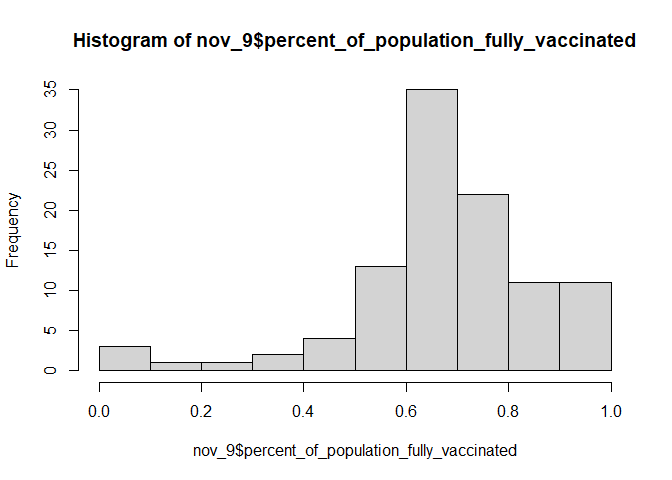
\includegraphics{class-17_files/figure-latex/unnamed-chunk-18-1.pdf}

\hypertarget{focus-on-ucsdla-jolla}{%
\subsection{Focus on UCSD/La Jolla}\label{focus-on-ucsdla-jolla}}

\begin{Shaded}
\begin{Highlighting}[]
\NormalTok{ucsd }\OtherTok{\textless{}{-}} \FunctionTok{filter}\NormalTok{(sd, zip\_code\_tabulation\_area }\SpecialCharTok{==} \StringTok{"92037"}\NormalTok{)}
\end{Highlighting}
\end{Shaded}

\begin{quote}
Q15. Using ggplot make a graph of the vaccination rate time course for
the 92037 ZIP code area
\end{quote}

\begin{Shaded}
\begin{Highlighting}[]
\NormalTok{ucsd }\SpecialCharTok{\%\textgreater{}\%} 
  \FunctionTok{ggplot}\NormalTok{(}\FunctionTok{aes}\NormalTok{(}\AttributeTok{x =}\NormalTok{ as\_of\_date, }\AttributeTok{y =}\NormalTok{ percent\_of\_population\_fully\_vaccinated)) }\SpecialCharTok{+}
  \FunctionTok{geom\_point}\NormalTok{()}\SpecialCharTok{+}
  \FunctionTok{geom\_line}\NormalTok{(}\AttributeTok{group =} \DecValTok{1}\NormalTok{)}\SpecialCharTok{+}
  \FunctionTok{ylim}\NormalTok{(}\FunctionTok{c}\NormalTok{(}\DecValTok{0}\NormalTok{,}\DecValTok{1}\NormalTok{)) }\SpecialCharTok{+}
  \FunctionTok{labs}\NormalTok{(}\AttributeTok{title =} \StringTok{"Vaccination Rate for La Jolla CA"}\NormalTok{, }\AttributeTok{y =} \StringTok{"Percent Vaccinated"}\NormalTok{, }\AttributeTok{x =} \StringTok{"Date"}\NormalTok{)}
\end{Highlighting}
\end{Shaded}

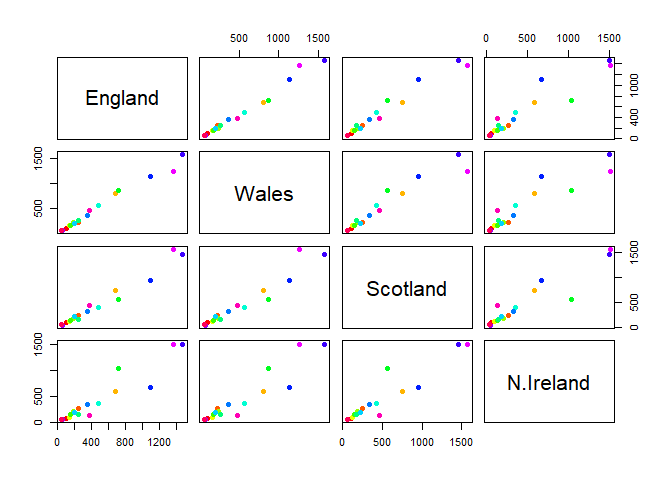
\includegraphics{class-17_files/figure-latex/unnamed-chunk-20-1.pdf}
\textgreater{} Q16. Calculate the mean ``Percent of Population Fully
Vaccinated'' for ZIP code areas with a population as large as 92037 (La
Jolla) as\_of\_date ``2021-11-16''. Add this as a straight horizontal
line to your plot from above with the geom\_hline() function?

\begin{Shaded}
\begin{Highlighting}[]
\NormalTok{sd }\SpecialCharTok{\%\textgreater{}\%} 
  \FunctionTok{filter}\NormalTok{(as\_of\_date }\SpecialCharTok{==} \StringTok{"2021{-}11{-}16"}\NormalTok{) }\SpecialCharTok{\%\textgreater{}\%} 
  \FunctionTok{filter}\NormalTok{(age5\_plus\_population }\SpecialCharTok{\textgreater{}=} \DecValTok{36144}\NormalTok{) }\SpecialCharTok{\%\textgreater{}\%} 
  \FunctionTok{summarise}\NormalTok{(}\AttributeTok{mean\_vaxrate =} \FunctionTok{mean}\NormalTok{(percent\_of\_population\_fully\_vaccinated))}
\end{Highlighting}
\end{Shaded}

\begin{verbatim}
##   mean_vaxrate
## 1    0.6744255
\end{verbatim}

\begin{Shaded}
\begin{Highlighting}[]
\NormalTok{ucsd }\SpecialCharTok{\%\textgreater{}\%} 
  \FunctionTok{ggplot}\NormalTok{(}\FunctionTok{aes}\NormalTok{(}\AttributeTok{x =}\NormalTok{ as\_of\_date, }\AttributeTok{y =}\NormalTok{ percent\_of\_population\_fully\_vaccinated)) }\SpecialCharTok{+}
  \FunctionTok{geom\_point}\NormalTok{()}\SpecialCharTok{+}
  \FunctionTok{geom\_line}\NormalTok{(}\AttributeTok{group =} \DecValTok{1}\NormalTok{)}\SpecialCharTok{+}
  \FunctionTok{ylim}\NormalTok{(}\FunctionTok{c}\NormalTok{(}\DecValTok{0}\NormalTok{,}\DecValTok{1}\NormalTok{)) }\SpecialCharTok{+}
  \FunctionTok{labs}\NormalTok{(}\AttributeTok{title =} \StringTok{"Vaccination Rate for La Jolla CA"}\NormalTok{, }\AttributeTok{y =} \StringTok{"Percent Vaccinated"}\NormalTok{, }\AttributeTok{x =} \StringTok{"Date"}\NormalTok{)}\SpecialCharTok{+}
  \FunctionTok{geom\_hline}\NormalTok{(}\AttributeTok{yintercept =} \FloatTok{0.6744255}\NormalTok{)}
\end{Highlighting}
\end{Shaded}

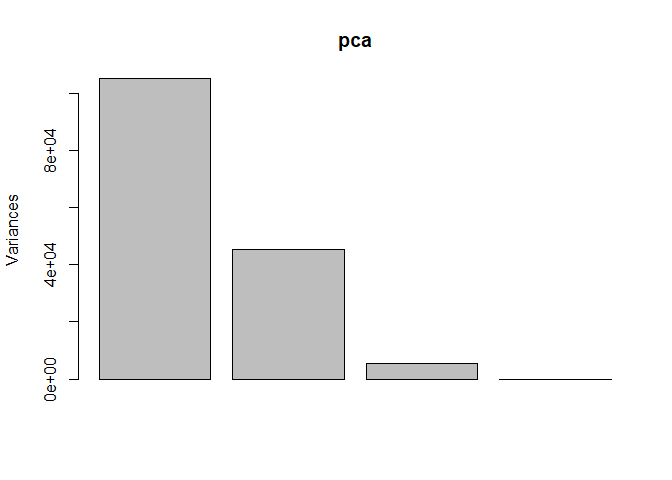
\includegraphics{class-17_files/figure-latex/unnamed-chunk-22-1.pdf}
\textgreater{} Q17. What is the 6 number summary (Min, 1st Qu., Median,
Mean, 3rd Qu., and Max) of the ``Percent of Population Fully
Vaccinated'' values for ZIP code areas with a population as large as
92037 (La Jolla) as\_of\_date ``2021-11-16''?

\begin{Shaded}
\begin{Highlighting}[]
\NormalTok{vax }\SpecialCharTok{\%\textgreater{}\%} 
  \FunctionTok{filter}\NormalTok{(as\_of\_date }\SpecialCharTok{==} \StringTok{"2021{-}11{-}16"}\NormalTok{) }\SpecialCharTok{\%\textgreater{}\%} 
  \FunctionTok{filter}\NormalTok{(age5\_plus\_population }\SpecialCharTok{\textgreater{}=} \DecValTok{36144}\NormalTok{) }\SpecialCharTok{\%\textgreater{}\%} 
  \FunctionTok{summarise}\NormalTok{(}\AttributeTok{min =} \FunctionTok{min}\NormalTok{(percent\_of\_population\_fully\_vaccinated), }\AttributeTok{median =} \FunctionTok{median}\NormalTok{(percent\_of\_population\_fully\_vaccinated), }\AttributeTok{mean =} \FunctionTok{mean}\NormalTok{(percent\_of\_population\_fully\_vaccinated), }\AttributeTok{sec\_qtr =}\NormalTok{ median}\SpecialCharTok{/}\DecValTok{2}\NormalTok{, }\AttributeTok{third\_qtr =} \DecValTok{3}\SpecialCharTok{/}\DecValTok{2}\SpecialCharTok{*}\NormalTok{(median),  }\AttributeTok{max =} \FunctionTok{max}\NormalTok{(percent\_of\_population\_fully\_vaccinated))}
\end{Highlighting}
\end{Shaded}

\begin{verbatim}
##        min   median      mean  sec_qtr third_qtr max
## 1 0.352891 0.666522 0.6646457 0.333261  0.999783   1
\end{verbatim}

\begin{quote}
Q18. Using ggplot generate a histogram of this data.
\end{quote}

\begin{Shaded}
\begin{Highlighting}[]
\NormalTok{vax }\SpecialCharTok{\%\textgreater{}\%} 
  \FunctionTok{filter}\NormalTok{(as\_of\_date }\SpecialCharTok{==} \StringTok{"2021{-}11{-}16"}\NormalTok{) }\SpecialCharTok{\%\textgreater{}\%} 
  \FunctionTok{filter}\NormalTok{(age5\_plus\_population }\SpecialCharTok{\textgreater{}=} \DecValTok{36144}\NormalTok{) }\SpecialCharTok{\%\textgreater{}\%} 
  \FunctionTok{ggplot}\NormalTok{(}\FunctionTok{aes}\NormalTok{(}\AttributeTok{x =}\NormalTok{ percent\_of\_population\_fully\_vaccinated)) }\SpecialCharTok{+}
  \FunctionTok{geom\_histogram}\NormalTok{()}
\end{Highlighting}
\end{Shaded}

\begin{verbatim}
## `stat_bin()` using `bins = 30`. Pick better value with `binwidth`.
\end{verbatim}

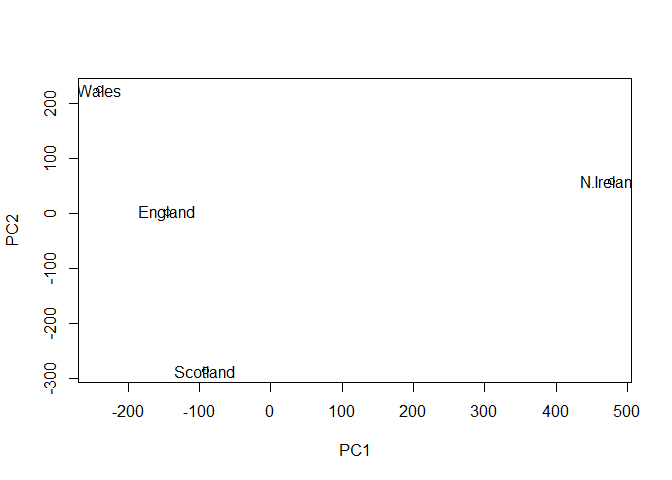
\includegraphics{class-17_files/figure-latex/unnamed-chunk-24-1.pdf}

\begin{quote}
Q19. Is the 92109 and 92040 ZIP code areas above or below the average
value you calculated for all these above?
\end{quote}

\begin{Shaded}
\begin{Highlighting}[]
\NormalTok{vax }\SpecialCharTok{\%\textgreater{}\%} \FunctionTok{filter}\NormalTok{(as\_of\_date }\SpecialCharTok{==} \StringTok{"2021{-}11{-}16"}\NormalTok{) }\SpecialCharTok{\%\textgreater{}\%}  
  \FunctionTok{filter}\NormalTok{(zip\_code\_tabulation\_area}\SpecialCharTok{==}\StringTok{"92040"}\NormalTok{) }\SpecialCharTok{\%\textgreater{}\%}
  \FunctionTok{select}\NormalTok{(percent\_of\_population\_fully\_vaccinated)}
\end{Highlighting}
\end{Shaded}

\begin{verbatim}
##   percent_of_population_fully_vaccinated
## 1                               0.521047
\end{verbatim}

Lower in ZIP 92040

\begin{Shaded}
\begin{Highlighting}[]
\NormalTok{vax }\SpecialCharTok{\%\textgreater{}\%} \FunctionTok{filter}\NormalTok{(as\_of\_date }\SpecialCharTok{==} \StringTok{"2021{-}11{-}16"}\NormalTok{) }\SpecialCharTok{\%\textgreater{}\%}  
  \FunctionTok{filter}\NormalTok{(zip\_code\_tabulation\_area}\SpecialCharTok{==}\StringTok{"92109"}\NormalTok{) }\SpecialCharTok{\%\textgreater{}\%}
  \FunctionTok{select}\NormalTok{(percent\_of\_population\_fully\_vaccinated)}
\end{Highlighting}
\end{Shaded}

\begin{verbatim}
##   percent_of_population_fully_vaccinated
## 1                                0.68863
\end{verbatim}

Greater in ZIP 92109

\begin{quote}
Q20. Finally make a time course plot of vaccination progress for all
areas in the full dataset with a age5\_plus\_population \textgreater{}
36144
\end{quote}

\begin{Shaded}
\begin{Highlighting}[]
\NormalTok{vax}\FloatTok{.36} \OtherTok{\textless{}{-}}\NormalTok{ vax }\SpecialCharTok{\%\textgreater{}\%} 
  \FunctionTok{filter}\NormalTok{(age5\_plus\_population }\SpecialCharTok{\textgreater{}} \DecValTok{36144}\NormalTok{) }
\NormalTok{vax}\FloatTok{.36} \SpecialCharTok{\%\textgreater{}\%} 
  \FunctionTok{ggplot}\NormalTok{(}\FunctionTok{aes}\NormalTok{(}\AttributeTok{x =}\NormalTok{ as\_of\_date,  }\AttributeTok{y =}\NormalTok{ percent\_of\_population\_fully\_vaccinated, }\AttributeTok{group =}\NormalTok{ zip\_code\_tabulation\_area)) }\SpecialCharTok{+}
  \FunctionTok{geom\_line}\NormalTok{(}\AttributeTok{alpha =} \FloatTok{0.2}\NormalTok{)}\SpecialCharTok{+}
  \FunctionTok{ylim}\NormalTok{(}\FunctionTok{c}\NormalTok{(}\DecValTok{0}\NormalTok{,}\DecValTok{1}\NormalTok{))}\SpecialCharTok{+}
  \FunctionTok{labs}\NormalTok{(}\AttributeTok{x =} \StringTok{"Date"}\NormalTok{, }\AttributeTok{y =} \StringTok{"Vaccination Rate"}\NormalTok{, }\AttributeTok{title =} \StringTok{"Vaccination Rates Across California"}\NormalTok{, }\AttributeTok{subtitle =} \StringTok{"In ZIP codes with populations greater than 36k"}\NormalTok{)}\SpecialCharTok{+}
  \FunctionTok{geom\_hline}\NormalTok{(}\AttributeTok{yintercept =} \FloatTok{0.6744255}\NormalTok{)}
\end{Highlighting}
\end{Shaded}

\begin{verbatim}
## Warning: Removed 176 row(s) containing missing values (geom_path).
\end{verbatim}

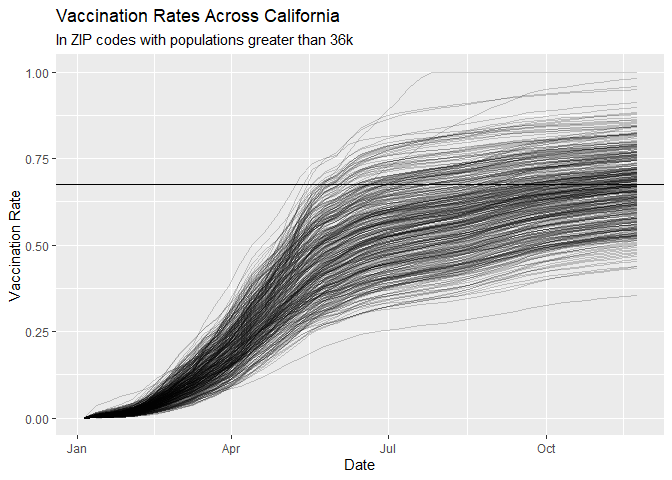
\includegraphics{class-17_files/figure-latex/unnamed-chunk-27-1.pdf}
\textgreater{} Q21. How do you feel about traveling for Thanksgiving and
meeting for in-person class next Week?

I know the decision has already been made but thanks for thinking about
our health after the traveling!

\end{document}
